\documentclass{article}


\usepackage{PRIMEarxiv}

\usepackage[utf8]{inputenc} % allow utf-8 input
\usepackage[T1]{fontenc}    % use 8-bit T1 fonts
\usepackage{hyperref}       % hyperlinks
\usepackage{url}            % simple URL typesetting
\usepackage{booktabs}       % professional-quality tables
\usepackage{amsfonts}       % blackboard math symbols
\usepackage{nicefrac}       % compact symbols for 1/2, etc.
\usepackage{microtype}      % microtypography
\usepackage{lipsum}
\usepackage{fancyhdr}       % header
\usepackage{graphicx}       % graphics
\graphicspath{{media/}}     % organize your images and other figures under media/ folder
\usepackage{amsmath}

%Header
\pagestyle{fancy}
\thispagestyle{empty}
\rhead{ \textit{ }} 

% Update your Headers here
\fancyhead[LO]{Running Title for Header}
% \fancyhead[RE]{Firstauthor and Secondauthor} % Firstauthor et al. if more than 2 - must use \documentclass[twoside]{article}



  
%% Title
\title{Speech separation in real time using deep learning architectures
%%%% Cite as
%%%% Update your official citation here when published 
\thanks{\textit{\underline{Citation}}: 
\textbf{Authors. Title. Pages.... DOI:000000/11111.}} 
}

\author{
  Jose A. Arango-Sánchez \\
  Intelligent Information Systems Lab - In2Lab \\
  Universidad de Antioquia \\
  Medellín, Colombia.\\
  \texttt{jose.arangos@udea.edu.co} \\
  %% examples of more authors
   \And
  Julián D. Arias-Londoño \\
  GAPS-SSR \\
  ETSIT-Universidad Politécnica de Madrid \\
  Madrid, Spain.\\
  \texttt{julian.arias@upm.es} \\
  %% \AND
  %% Coauthor \\
  %% Affiliation \\
  %% Address \\
  %% \texttt{email} \\
  %% \And
  %% Coauthor \\
  %% Affiliation \\
  %% Address \\
  %% \texttt{email} \\
  %% \And
  %% Coauthor \\
  %% Affiliation \\
  %% Address \\
  %% \texttt{email} \\
}


\begin{document}
\maketitle


\begin{abstract}

\end{abstract}


% keywords can be removed
\keywords{ Speaker Separation \and Single-Channel \and Real-Time \and Similitude Speakers \and Speech Embeddings \and Conv-TasNet \and Corpus Phone Calls Spanish}


\section{Introduction}



\section{Base architecture}
Currently, most of the approaches (architectures) used for speaker separation are based on deep neural networks. Basically, these architectures are trained with a large number of audios, composed of a mixture and the different isolated sources. The neural network during the training process, must produce an output for each source (estimated source), and then compare each output with the true isolated source (real source). This comparison is used to update the weights of the network to generate better results in future iterations. This process is known as back-propagation.

Since it is necessary to have the mixture and the sources, many of the speaker separation systems are supervised machine learning systems. In order to obtain good results, it is important to have a considerable amount of training data.

In the following we will describe in detail one of the architectures that set a milestone in the field of speaker separation:

\subsection{Conv-TasNet}
Conv-Tasnet, is a fully convolutional time domain audio separation network with an End-to-End approach \cite{luo2019conv}.

This architecture is composed of 3 key components, which are shown in Figure \ref{fig:tasnet_block}. Globally, this architecture has an Encoder, which generates a high-dimensional representation of segments of the mixture waveform. Then, we have a Separation component, which computes a mask for each of the target sources. Finally, a Decoder reconstructs the Waveforms of the sources based on the masked features \cite{luo2019conv}.

\begin{figure}[!h]
    \centering
    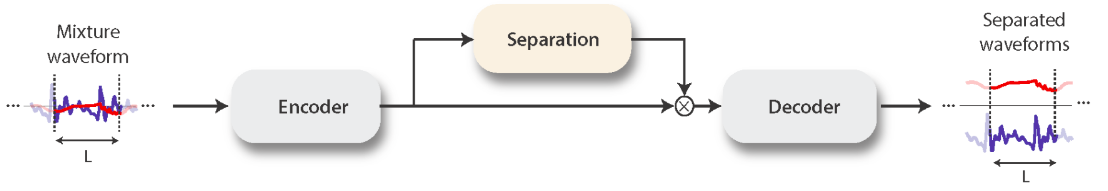
\includegraphics[scale=0.38]{Figures/arquitecturas/tasnet_block.png}
    \caption{Key components of the Conv-TasNet architecture. Taken from \cite{luo2019conv}.}
    \label{fig:tasnet_block}
\end{figure}

\begin{enumerate}
    \item Encoder
    It transforms short segments of the mixture waveform into an intermediate feature space. For this, it use a linear encoder, that it replaces the STFT used for feature extraction with a data-driven representation, which is optimized in conjunction with an End-to-End training paradigm.
    
    
    \item Separation
    This module estimates a multiplicative function (masks) for each source at each time step. These masks are obtained through a temporal convolutional network (TCN), which is formed by 1-D stacked dilated convolutional blocks. This allows the network to model the long-term dependencies of the speech signal while maintaining a small model size. Finally, speaker separation is achieved by applying a set of weighting functions (masks) to the encoder output.

    \item Decoder
    Reconstructs the waveform using a linear decoder, which plays the role of the iSTFT. the role of the iSTFT.
    
\end{enumerate}
As shown in Figure \ref{fig:system_flowchart}, both the Encoder and the Decoder are composed of a 1-D convolution block, which is described in Figure \ref{fig:block_conv}. Where each block consists of a 1×1 convolution operation followed by a depthwise convolution operation, with a nonlinear activation function and a normalization added between each of the two convolution operations. Finally, two 1 × 1-conv linear blocks serve as residual path and jump connection path for the next block, respectively \cite{luo2019conv}.

\begin{figure}[!h]
    \centering
    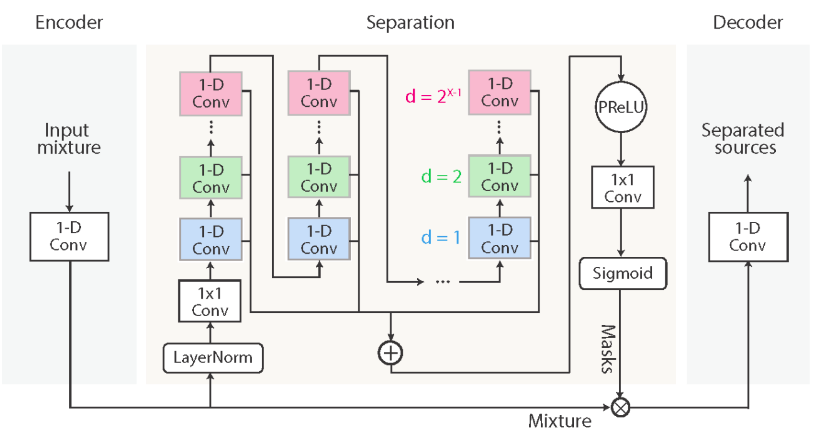
\includegraphics[scale=0.5]{Figures/arquitecturas/B.System_flowchart.png}
    \caption{Conv-TasNet architecture flowchart. Taken from \cite{luo2019conv}.}
    \label{fig:system_flowchart}
\end{figure}

The separation module, which can be seen in Figure \ref{fig:system_flowchart}, is in charge of estimating the masks based on the encoder output. This module is composed of different layers, which in turn contain different 1-D convolutional blocks. Each 1-D convolutional block has different dilation factors, which increase exponentially. This guarantees a sufficiently large temporal context window, thus taking advantage of the long-range dependencies of the speech signal. The different colors of the 1-D convolutional blocks denote different dilation factors \cite{luo2019conv}.


\begin{figure}[!h]
    \centering
    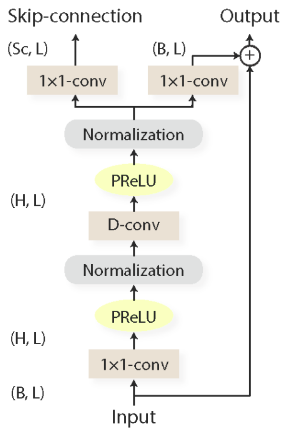
\includegraphics[scale=0.6]{Figures/arquitecturas/C.1-D_Conv_block_design.png}
    \caption{Structure of a convolutional block (1-D Conv) ConvTasNet architecture. Taken from \cite{luo2019conv}.}
    \label{fig:block_conv}
\end{figure}

The cost function used by the Conv-TasNet model is the scale-invariant Signal-to-Noise Ratio (SI-SNR). The training objective of this end-to-end system is to maximize this measure. The SI-SNR is defined by:

\begin{equation}
    \text{ SI-SNR : }=10 \log _{10} \frac{\left\|\mathbf{s}_{\text {target}}\right\|^{2}}{\left\|\mathbf{e}_{\text {noise }}\right\|^{2}}
\end{equation}

Where $\mathbf{s}_{\text {target }}$ and $\mathbf{e}_{\text {noise }}$,  are given by:

\begin{equation}
    \mathbf{s}_{\text {target }}:=\frac{\langle\hat{\mathbf{s}}, \mathbf{s}\rangle \mathbf{s}}{\|\mathbf{s}\|^{2}}
\end{equation}

\begin{equation}
    \mathbf{e}_{\text {noise }}:=\hat{\mathbf{s}}-\mathbf{s}_{\text {target }}
\end{equation}
Where $\hat{\mathbf{s}} \in \mathbb{R}^{1 \times T}$ and $\mathbf{s} \in \mathbb{R}^{1 \times T}$ are the estimated source and true source, respectively, and
$\|\mathbf{s}\|^{2}=\langle\mathbf{s}\mathbf{s}\rangle$ denotes the signal power. Scale-Invariant is guaranteed by normalizing $\hat{s}$ and $s$ to zero mean before calculation \cite{luo2019conv}.

Finally, the Conv-TasNet system significantly outperforms masking methods based on time-frequency representations for two- and three-speaker mixtures. In addition, Conv-TasNet outperforms several ideal masks of time-frequency magnitude in the separation of two-speaker speech as assessed by both objective measures of distortion and subjective quality assessment. Finally, Conv-TasNet has a significantly small model size (5.1 Million parameters) and minimal latency compared to other models, making it a suitable solution for real-time speech separation applications \cite{luo2019conv}.




\section{Similitude between speakers}

\subsection{Speech Embeddings}
\subsubsection{Wav2Vec 2.0}
\subsubsection{Pyannote}

\section{Conv-TasNet modified}

\section{Experiments}
\subsection{Corpus phone calls}

\section{Results}
\subsection{Conv-TasNet}
\subsection{Conv-TasNet modified}

\section{Deploy}

\section{Conclusion}


\section*{Acknowledgments}
This was was supported in part by......

%Bibliography
\bibliographystyle{unsrt}  
\bibliography{references}  


\end{document}
